\begin{comment}
	### AI LEARNING GOALS
	- Running X Model
	- Able to use SDK; CLI
	- (Optional) Understanding Neural Networks better
	### Research Sources
	- Person-Cours
	- 3-hours metric cours
	- Azure Certificate: DP-100
	<- Documentation, that I can manage learn those courses
	#### How to Doc
	- LaTex Deep dive -> Take what is usefull or relevant for other people i Markdown (But not before)
	- Emmy_ML_One: Code Repos <- Other Repos in Notes_DSci
	- Topics to explain
	- Design Explation: AutoML, Designer as a first approach -> putting it all into one model
	- Explanation SDK, CLI
	--------------------------------------------------------
	
	# General enviroment file (local enviroments)		
	
	# Learning Basics for SDK, CLI
	- Basic Doc understanding -> LaTex
	- Simple ML-Model Example (Either by Mircosoft Doc or Perscon Example)
	- Start Experiment
	- Train a Model on different compute targets
	- Log Metrics
	- (Maybe) Register Model
	- Test Model
	
	# Exended DevOps Setup
	- Unity data sanity tests
	- Model version
	- Model evaluation
	- (Optional: Deployment)
	
	# automatic CI flake8, mypy (at least) for model script
	- setup envirnoment files, that the ci pipeline can use them,
	- setup ymal file to run CI pipeline for code review test.
	
	# Learn More about Neural Network
\end{comment} 

\section{azureml-core (Python SDK)}
% I want to be this guy, who builds with his team an increatiable A.I: system for munich.

\subsection{Connect to Workspace}
A workspace is a resource, which is tied (child) to a subscription and a resource group. A workspace links the different object to run a \gls{ML} model: Experiment, Training, Deployment. A workspace comes with a \gls{SDK} to interactive with.\\

To connect to the workspace, the constructor requires different parameters
\begin{lstlisting}[style=python]
	Workspace(
	subscription_id, resource_group, workspace_name,
	auth=None,
	_location=None,
	_disable_service_check=False,
	_workspace_id=None,
	sku='basic',tags=None, _cloud='AzureCloud'
	)
\end{lstlisting} 


\begin{comment}
\begin{figure}[H]
	\centering
	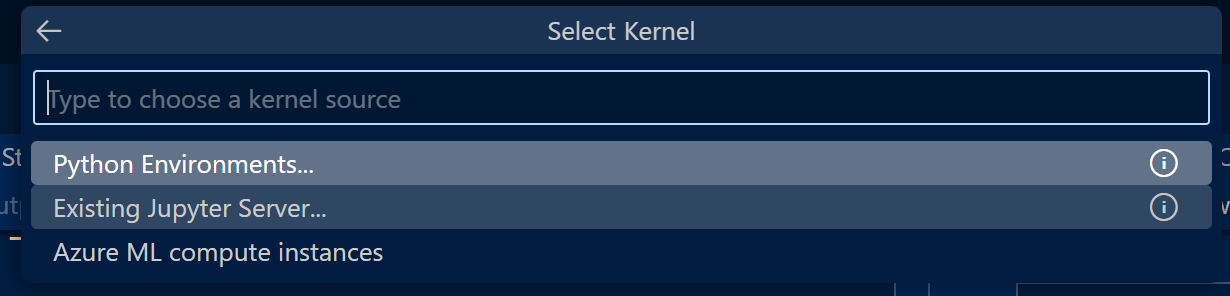
\includegraphics[scale = 0.3]{attachment/chapter_AML/Scc001}
	\caption{Connect to the workspace: Select kernel}
\end{figure}

We started, with writing the configuration file.
A started with opening jupter notebook and den selecting the kernel. And a kernel was installed on the compute cluster.
The authen

\\
auth
ServicePrincipalAuthentication or InteractiveLoginAuthentication or MsiAuthentication
default value: None
The authentication object. For more details, see https://aka.ms/aml-notebook-auth. If None, the default Azure CLI credentials will be used or the API will prompt for credentials.


\begin{lstlisting}[style=python]
	from azureml.core import Workspace
	ws = Workspace.create(name='myworkspace',
	subscription_id='<azure-subscription-id>',
	resource_group='myresourcegroup',
	create_resource_group=True,
	location='eastus2'
	)
	
	for i in range(n):
	print('i = ', i)
\end{lstlisting}


\end{comment}



